\documentclass[letter]{llncs}

\newcommand{\figshrink}{\vspace{-.6cm}}
%\newcommand{\figshrinkend}{\vspace{-.4cm}}
\newcommand{\figshrinkend}{}
\usepackage{amssymb}
\setcounter{tocdepth}{3}
\usepackage{graphicx}
\usepackage{amsmath}
\usepackage{algpseudocode}% http://ctan.org/pkg/algorithmicx
\usepackage{algorithm}
\usepackage{amsmath}
\usepackage{url}
\urldef{\mailsa}\path|{alfred.hofmann, ursula.barth, ingrid.haas,
frank.holzwarth,|
\urldef{\mailsb}\path|anna.kramer, leonie.kunz, christine.reiss, nicole.sator,|
\urldef{\mailsc}\path|erika.siebert-cole, peter.strasser, lncs}@springer.com|  
\newcommand{\Tr}{\ensuremath{\mathsf{TrS}}}
\newcommand{\TrR}{\ensuremath{\mathsf{TrR}}}
\newcommand{\TrA}{\ensuremath{\mathsf{Cond}}}
\renewcommand{\a}[1]{\ensuremath{\mathsf{#1}}}
\newcommand{\concat}{\ensuremath{\mathop{+\!\!+}}}
%\newcommand{\figshrinkend}{\vspace{-.4cm}}
\newcommand{\secshrink}{\vspace{-.5cm}}
\newcommand{\secshrinkbegin}{\vspace{-.2cm}}
\newcommand{\subsecshrink}{\vspace{-.5cm}}
\newcommand{\subsecshrinkbegin}{\vspace{-.2cm}}
\setlength{\abovecaptionskip}{1ex}
\setlength{\belowcaptionskip}{1ex}
\setlength{\floatsep}{1ex}
\setlength{\textfloatsep}{1ex}
% \usepackage{times}
\usepackage{amssymb}
\setcounter{tocdepth}{3}
\usepackage{graphicx}
\usepackage{amsmath}
% \usepackage[options]{algorithm2e}
% \usepackage{algorithm}% http://ctan.org/pkg/algorithms
\usepackage{algpseudocode}% http://ctan.org/pkg/algorithmicx
\usepackage{algorithm}

\makeatletter
\renewcommand{\ALG@beginalgorithmic}{\small}
\algrenewcommand\algorithmicindent{0.5em}%
\makeatother
\usepackage[caption=false,font=footnotesize]{subfig}
\usepackage{url}
\urldef{\mailsa}\path|{alfred.hofmann, ursula.barth, ingrid.haas,
frank.holzwarth,|
\urldef{\mailsb}\path|anna.kramer, leonie.kunz, christine.reiss, nicole.sator,|
\urldef{\mailsc}\path|erika.siebert-cole, peter.strasser, lncs}@springer.com|  
\usepackage{listings}
\usepackage{enumerate}
\usepackage{textcomp}
\DeclareMathSizes{10}{10}{9}{9}
\usepackage{algpseudocode}% http://ctan.org/pkg/algorithmicx

\begin{document}

\title{Property Specification Made Easy: Harnessing the Power of Model Checking in UML designs}

\author{Daniela Remenska\inst{1,3}
\and Tim A.C. Willemse\inst{2} \and Jeff Templon\inst{3} \and\
Kees Verstoep\inst{1} \and Henri Bal\inst{1}}
%
% (feature abused for this document to repeat the title also on left hand pages)

% the affiliations are given next; don't give your e-mail address
% unless you accept that it will be published
\institute{Dept. of Computer Science, VU University Amsterdam, The Netherlands
\and
Dept. of Computer Science, TU Eindhoven, The Netherlands
\and
NIKHEF, Amsterdam, The Netherlands
}

\toctitle{Lecture Notes in Computer Science}
\tocauthor{Authors' Instructions}
\maketitle

\begin{abstract}
Early discovery of design errors which can lead to deadlocks or race conditions is 
challenging in concurrent software development. 
In the last decades, more rigorous
methods and tools for modeling and formal analysis have been developed. 
Although approaches for automatically generating formal models from system designs have 
been proposed, another serious obstacle for adopting model checking tools in industry
is the formulation of application-specific properties to be checked. 
This requires expertise in temporal logic, regardless of the verification tool used.
To bring the process of correctly eliciting functional properties closer to software 
designers, we introduce PASS, a Property ASSistant wizard developed 
as an Eclipse plugin. Our starting point was the well-established property pattern system,
which we extended with new property templates, to capture variations not covered 
in the original classification. PASS instantiates pattern templates using three notations: a natural language summary, a $\mu$-calculus formula
and a UML sequence diagram depicting the desired behavior. Most approaches to date 
have focused on LTL, which is a state-based formalism. On the other hand,
 $\mu$-calculus is event-based, making it a good match for sequence diagrams, where communication between
 components is depicted. 
Moreover, such communication is data-dependent, so we introduce
the possibility to define data quantifiers, to express complex properties in a concise manner.
To cope with state-space explosion, we provide one additional notation: a monitor for on-the-fly model checking, or bug hunting.
We revisit a case study from the Grid domain, using PASS to obtain the
formula and monitor for checking the property with mCRL2.
% \keywords{property specification, model checking, UML, sequence diagrams, modal
% $\mu$-calculus, property patterns}
\end{abstract}
\section{Introduction}
\label{sec:Introduction}
One of the challenges in concurrent software development is early discovery of design errors which can lead to deadlocks or race conditions.
Traditional testing does not always expose such problems in complex distributed applications. Performing more rigorous formal analysis, like model-checking, 
typically requires a model which is an abstraction of the system.
In the last decades, methods and tools
for modeling and formal analysis have been developed. Some of the leading model checking tools include SPIN, nuSMV, CADP and mCRL2. 
Despite the research effort, these tools are still not widely accepted in the software industry. One problem is the lack of expertise and
the necessary time investment in the development cycle, for becoming proficient in
the underlying mathematical formalisms used for describing the models. 
To bridge the gap between industry-adopted methodologies based on UML software
designs, and model-checking tools and languages, in~\cite{DBLP:dblp_conf/nfm/RemenskaTWHVCB13} we devised 
an automated transformation methodology for verification of UML
models, based on sequence and activity diagrams. Our prototype is able to produce
a formal model into the mCRL2 process algebra language~\cite{FormalLanguagemCRL2}, and feed model-checking traces back into any modeling
tool, without the user having to leave the UML domain. We chose mCRL2 because of its strong tool support and rich data types compared to other languages.
%mention why we chose SDs!
Figure~\ref{fig:approach} gives an overview of our approach and implemented toolchain.
Although the mCRL2 toolset automatically discovers deadlocks, model checking
for application-specific properties requires the use of modal $\mu$-calculus~\cite{Groote05model-checkingprocesses}. In principle, regardless of the formal language and tool choice for writing the model, these properties 
are specified as formulas in some temporal logic formalism, such as Linear Temporal Logic (LTL), Computation Tree Logic (CTL), Quantified Regular Expressions (QRE) or $\mu$-calculus.
\begin{figure}[!t]
\centering
\figshrink
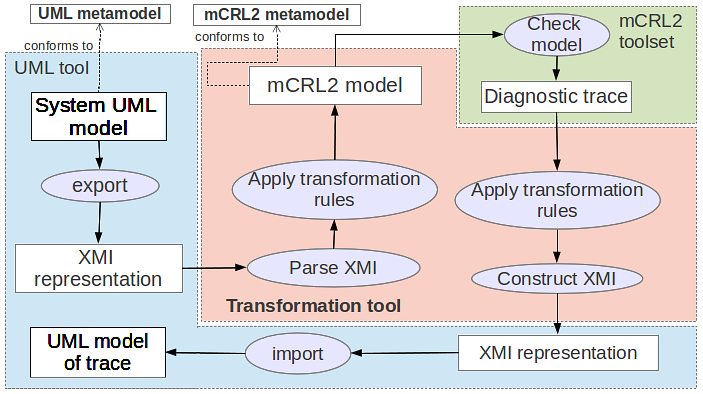
\includegraphics[width=0.7\linewidth,keepaspectratio=true]{./Approach.png}
\caption{Automated verification of UML models}
\label{fig:approach}
\figshrinkend
\end{figure}
The level of sophistication and mathematical background required for using such formalisms is yet another obstacle for adopting formal methods. 
In practice, software requirements are written in natural language, and often contain ambiguities, making it difficult even for experienced 
practitioners to capture them accurately with temporal logic. There are subtle, but crucial details which are often overlooked and 
need to be carefully considered in order to distill the right formula.

% just mention here the patterns, the fact that there are 3 categories of approaches
% tackling the problem, the general deficiencies of these approaches and how we want to
% take the best of all worlds; 
Based on investigation of more than 500 properties coming from different domains, and specified in several formalisms, a pattern-based classification
was developed in~\cite{Dwyer:1999:PPS:302405.302672}. The authors observed that almost all the surveyed properties
can be mapped into one of several property patterns. Each pattern is a
high-level, formalism-independent abstraction that captures a
commonly occurring requirement. These patterns can be instantiated with specific
events or states and then mapped to several different formalisms for model
checking tools. Their hierarchical taxonomy is based on the idea that each
pattern has a \emph{scope}, which defines the extent of program execution over
which the pattern must hold, and a \emph{behavior}, which describes the intent of the pattern. The pattern
system identifies 5 scopes and 11 behavior variations that can be
combined to create 55 different property templates. Examples of scopes are: globally,
before an event or state occurs, after an event or state occurs.
Examples of behavior classification are: absence (an event or state should never
occur during an execution), precedence (an event or
state always occurs before another one), 
or response (the occurrence of a an event or state must be followed by
another event or state), capturing a cause-effect relation.
Although the patterns website~\cite{PSP} contains a collection of mappings for
different target formalisms, such as LTL, CTL, QRE and Graphical Interval Logic, which can be considered helpful,
practitioners have to fully understand the provided solutions before they can
select and apply the appropriate ones in practice.

To mitigate the problem, several approaches~\cite{Smith02propel:an,konrad2005facilitating,Mondragon_prospec} propose conversational tools for
elucidating properties, based on the property patterns. These tools guide users in selecting the appropriate pattern
for the property in mind, and optionally produce a formula in some target temporal logic. 
Another category of approaches~\cite{Ziemann02anextension,Flake03formalsemantics,Ackermann:2006:LOS:2135315.2135339} deal with temporal extensions 
of the Object Constraint Language (OCL), as means to specify system
properties. OCL is a declarative textual language for describing invariants for
classes and pre- and postconditions of operations. Although it forms an integral
part of UML, it lacks means to specify constraints over the dynamic behavior
of a model. Finally, a third class of approaches~\cite{Autili:2007:GSS:1290845.1290859,Lee97agraphical,Smith:2001:ECG:882477.883639,Knapp:2006:MCU:1762828.1762836,Lilius99vuml:a,Kugler:2005:TLS:2140653.2140692,MVPSA} tackle the property
specification problem by proposing graphical notations for specifying properties.

The objective of this work is to simplify the process of correctly eliciting
functional requirements, without the need of expertise in temporal logic. 
First, we introduce PASS, a Property ASSistant which guides and facilitates the process of deriving
system properties. Our starting point was the pattern system,
which we extended with over 40 new property templates, to capture variations not covered 
in the original classification. Our strong motivation was to stay
in the same UML development environment, rather than use an external helper tool for this.
It should increase the tool accessibility by allowing software engineers to remain focused in the realm of UML designs.
In addition, a tight bond between elements of the design and instances of the property template is kept, such that, if the 
design is changed, these changes can be easily propagated in the property template placeholders. 
To this end, we use the standard MDT-UML2~\cite{MDTUML2} Eclipse modeling API. Our tool is developed as an Eclipse plugin.
Second, the pattern templates instantiated with PASS have three notations: a natural language summary, a $\mu$-calculus formula
and a UML sequence diagram depicting the desired behavior. Most approaches to date 
have focused on LTL, which is a state-based temporal logics formalism. On the other hand,
 $\mu$-calculus is event-based, and as such is a good match for the sequence diagrams notation. 
These events can represent methods calls or asynchronous communication between distributed components.
Moreover, such communication is data-dependent, which is why we introduce
the possibility to define quantifiers, to express complex properties in a concise manner, e.g., every
element of a certain type must fulfill a certain property. 
Unlike LTL or CTL,  $\mu$-calculus is powerful enough
to achieve this in a natural way. Third, to cope with state-space explosion,
we provide one additional automatically-generated notation: a monitor for on-the-fly model checking, or bug hunting.
We interpret a sequence diagram as an observer of the message exchanges in the system.
This helps in avoiding generation of those parts of the state space for which it is 
certain that they do not compose with the property monitor. The state space
generation is thus property driven, and stops as soon as an error is found.
Finally, we revisit a case study we did previously in~\cite{DBLP:dblp_conf/nfm/RemenskaTWHVCB13}, this time
using the PASS tool to automatically obtain the formula and monitor for checking the property in mCRL2.

This paper is structured as follows: in Section~\ref{sec:RelatedWork} we
 survey the most relevant related approaches,
and outline their advantages and shortcomings. Section~\ref{sec:Preliminaries} briefly introduces the
syntax and semantics of mCRL2, $\mu$-calculus and UML sequence diagrams.
We describe our approach in Section~\ref{sec:Approach}.
In Section~\ref{sec:CaseStudy} we apply it on a case study from the Grid domain, and we conclude in Section~\ref{sec:Conclusions}.
\section{Related Work}
\label{sec:RelatedWork}
In~\cite{Smith02propel:an} the authors developed PROPEL, a tool for guiding users in 
selecting the appropriate template. Recognizing that there are subtle aspects
not covered by the original patterns, such as what happens in a response
property if the cause occurs multiple times before the effect takes place,
they extended them with variants. The resulting templates 
are represented using disciplined natural language and finite state automata. 
PROPEL does not support the universality, bounded existence, and the chain patterns. It also 
does not produce a formula in any of the commonly used temporal logic formalisms.
In a similar manner, SPIDER~\cite{konrad2005facilitating} and 
Prospec~\cite{Mondragon_prospec} offer assistance in the specification process, and extend the original patterns
with compositional ones that are built up from combinations of more basic patterns. 
Unfortunately, we could not find SPIDER online, and the version of Prospec that we tested (Fig.~\ref{fig:Prospec}) produces only 
formulas in Future Interval Logic, not LTL as stated in the work.

Of the approaches that deal with temporal extensions of OCL,~\cite{Ziemann02anextension}
introduces the @pre and @next temporal modifiers for specification of past and future state-oriented constraints. 
By means of UML Profiles,~\cite{Flake03formalsemantics}
proposes another OCL extension for real-time constraints. They claim to be able to describe all the existing 
patterns in these OCL expressions. Their starting point for model descriptions are UML state machines.
To simplify constraint definition with OCL, in~\cite{Ackermann:2006:LOS:2135315.2135339} the authors 
propose to use specification patterns for which OCL constraints can be generated automatically.
The behavioral specification of software components refers to interface specifications,
which are not really dynamic views. This work does not yet introduce means to specify temporal properties.
Resembling an OO programming language, OCL constraints can become quite dense and cryptic, and editing 
them manually is error-prone. Another problem is the extent to which designers are familiar with this language.
\begin{figure*}[t!]
  \centering
  \subfloat{\label{fig:Prospec}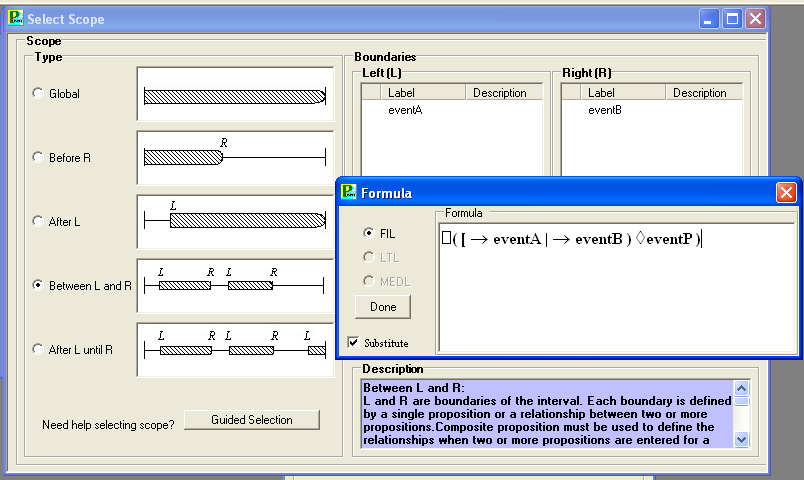
\includegraphics[width=0.73\linewidth]{./Prospec.png}}    
  \hfill
  \subfloat{\label{fig:Charmy}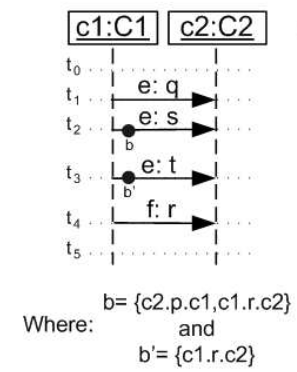
\includegraphics[width =0.26\linewidth]{./Charmy.png}}
  \caption{Left: Prospec tool; Right: CHARMY PSC graphical notation}
\end{figure*}

Graphical notation approaches come closest to the realm of modeling the system behavior.
%closest to our work...
The CHARMY approach~\cite{Autili:2007:GSS:1290845.1290859} presents a scenario-based visual language called 
Property Sequence Charts (PSC), where a property is seen as a relation on a set of exchanged
system messages. The language borrows concepts from UML 2.0 Sequence Diagrams, and its expressiveness
is measured with the property patterns. SPIN is used as a backend for model checking of
the Buchi automata~\cite{Giannakopoulou:2001:AVT:872023.872506}, which are 
an operational representation for LTL formulas generated automatically with this approach.
The PSC notation uses textual restrictions for past and future events, placed as circles directly on the message arrows (Fig.~\ref{fig:Charmy}).
Such a mix of textual and visual representation of message communication
within a diagram can be error-prone. Additionally, asynchronous communication is not supported.
Furthermore, even though concepts from UML are borrowed, CHARMY is a stand-alone framework for architectural descriptions,
not inter-operable with UML tools, and as such has limited usefulness in industrial context.
Another graphical language is proposed in~\cite{Lee97agraphical}, where formulas
are represented as acyclic graphs of states and temporal operators as nodes.
While they manage to hide the formalism from the user by generating LTL formulas, 
their notation is still very close to an actual temporal logic formula.
The TimeLine Editor~\cite{Smith:2001:ECG:882477.883639} also attempts to simplify the formalization of certain
kinds of requirements. Response formulas are depicted in timeline diagrams by specifying temporal relations among events and constraints. 
The timeline specification is automatically converted into a Buchi automaton, amenable to model checking with SPIN.
Unfortunately the tool is no longer available.
HUGO/RT~\cite{Knapp:2006:MCU:1762828.1762836} is a tool for model checking UML 2.0 interactions 
against a model composed of message-exchanging state machines. The interactions represent the desired properties,
and are translated together with the system model into Buchi automata for model checking with SPIN.
The approach uses some inner format for textual representation of UML interactions (rather than
the standard XMI), and the version we tested does not support asynchronous messages, or combined fragments.
vUML~\cite{Lilius99vuml:a} is a tool for automatic verification of UML models comprising state machines.
However, properties must be specified in terms of undesired scenarios, which is not always convenient.
This is because the verification is based on checking whether it is possible to reach error states, which must be manually specified by the user.
Live Sequence Charts (LSC) are also used~\cite{Kugler:2005:TLS:2140653.2140692,MVPSA} as a graphical formalism for expressing behavioral properties.
Their elements allow to distinguish between possible (cold) and mandatory (hot) behavior.
In both approaches, Buchi automata and a LTL formulas are generated automatically from the diagrams.
However, UML 2.0 sequence diagrams already borrow many concepts from LSC, by introducing the \emph{assert} and \emph{negate} fragments
to capture mandatory and forbidden behavior. On the other hand, being an older graphical notation, LSC lacks many UML features.

\section{Preliminaries}
\label{sec:Preliminaries}
%\subsection{Property Patterns}

\subsection{Brief Introduction to mCRL2 and $\mu$-calculus}
mCRL2 is a process algebra language for specification and analysis of concurrent systems. 
Our choice of mCRL2 as a formal language is motivated by its rich set of 
abstract data types as first-class citizens, as well as its powerful toolset for analysis, simulation, and visualization of specifications. 
The syntax of mCRL2 is given by the following BNF grammar:
\vspace{-7 pt}
$ \\ $
$ \\ $
$p ::= a(d_1,\dots,d_n)\ |\ \tau |\ \delta\ |\ p+p\ |\ p.p\ |\ p||p\ |\sum_{d:D}p\ |\ c\rightarrow p\diamond p$
\vspace{4 pt}
$ \\ $
Actions are the basic ingredients for models. They represent some observable
atomic event. An action $a$ of a process may have a number of data arguments  \begin{math}d_1,...,d_n\end{math}.
The action ${\tau}$ denotes an internal step, which cannot be observed from the external world. 
Non-deterministic choice between two processes
is denoted by the “+” operator. Processes can be composed sequentially and in parallel by means of ``.'' and
``${||}$''. The sum
operator $\sum_{d:D}p$ denotes (possibly infinite) choice among
processes parameterized by $d$. $c\rightarrow p\diamond p$ is a conditional
process, and depending on the value of the boolean expression $c$, the first or second operand is selected.
This allows for modeling of systems whose behavior is data-dependent.

To enforce synchronization, the allow operator ${\Delta_H(p)}$ specifies the set of actions $H$ that are allowed
to occur. To show possible communications in a system and the resulting actions, the communication operator
${\Gamma_C(p)}$ is used. The elements of set $C$ are so-called multi-actions of the form $a_1\ |\ a_2\ |\ \dots |\ a_n \rightarrow c$, which intuitively
means that action $c$ is the result of the multi-party synchronization of actions $a_1 , a_2 , \dots $ and $a_n$.
There are a number of built-in data types in mCRL2, such as (unbounded) integers, (uncountable)
reals, booleans, lists, and sets. 
Furthermore, by a \textbf{sort} definition one can define a new data type. A new process
is declared by \textbf{proc}.

The semantics associated with the mCRL2 syntax is a Labeled Transition System (LTS)
system that has multi-action labeled transitions, which can carry data parameters. The language used by the mCRL2
toolset for model-checking specific properties is the modal
$\mu$-calculus~\cite{Emerson97modelchecking}. This formalism stands out from most modal and temporal logic formalisms with respect to its
expressive power. Temporal logics like LTL, CTL and CTL* all have translations into $\mu$-calculus,
witnessing its generality. This expressiveness comes at a cost: very complex formulas with no intuitive and apparent interpretation can be coined. 
The syntax of a $\mu$-calculus formula is defined by the following grammar:
\[
\begin{array}{ll}

\phi_1 & ::= true \mid false \mid \phi\wedge\phi \mid \phi\vee\phi \mid [\rho]\phi \mid \langle\rho\rangle\phi \mid \mu Z\ldotp\phi \mid \nu Z\ldotp\phi \\
\rho & ::= \alpha \mid nil \mid \rho\cdot\rho \mid \rho^* \mid \rho^+ \\
\alpha & ::= \alpha\cup\alpha \mid \alpha\cap\alpha \mid\neg\alpha \mid true\\
\end{array}
\]
Properties represented by $\phi$ can be combined using the standard Boolean connectives.
The formula $\phi_1\wedge\phi_2$ is true whenever both $\phi_1$ and $\phi_2$ are true.
$\rho$ represents a set of sequences of actions, while $\alpha$ stands for a set of actions.
To describe a sequence of actions $\rho$, the concatenation $\rho\cdot\rho$ and iteration $\rho^*$ (possibly infinite sequences) operators can be used.
Union and intersection of sets of actions is denoted by $\cup$ and $\cap$ respectively. 
The notation $\neg\alpha$ denotes the complement of the set of actions $\alpha$ with respect to the set of all actions. 
The set of actions characterized by $\emph{true}$ is the entire set of actions present in the model, while \emph{nil} represents empty, i.e., no action.

The $\square$ (\emph{must}) and $\Diamond$ (\emph{may}) modalities  have the following semantics:
a state of the LTS satisfies $\langle R \rangle\phi$ iff there is at least one transition sequence 
starting at that state, satisfying R, and leading to a state satisfying $\phi$;
$[R]\phi$ is satisfied iff all sequences starting at that state and satisfying R, 
lead to states satisfying  $\phi$.
In other words, $[R]\phi$ describes that $\phi$ holds in all states that can be reached by a sequence in R,
while $\langle R \rangle\phi$ describes that $\phi$ holds in some state that can be reached by a sequence in R.
Remember that $[a]\phi$ is trivially satisfied for states with no “\emph{a}”-transitions.
Combined with these modalities, the least ($\mu X\ldotp f(X)$) and greatest
($\nu X\ldotp f(X)$) fixpoints permit reasoning about finite and infinite runs
of a system in a recursion-like manner.
For example, we can read $\mu X\ldotp\phi\vee\langle\alpha\rangle X$ as: X is
the smallest set of states such that a state is in X
iff $\phi$ holds in that state or there is an $\alpha$-successor in X. 
On the other hand, 
Conversely, $\nu X\ldotp\phi \wedge[\alpha]X$ is the largest set of states such that a state is in X iff
$\phi$ holds in that state and all of its $\alpha$-successors are in X.

Finally, a strong asset of $\mu$-calculus are the universal (\emph{forall}) and existential (\emph{exists}) quantifiers over possibly-infinite data types.
For example, \emph{forall n:Nat.$\langle$read(n)$\rangle$true} asserts that a process can execute a read action with every natural number as a parameter;
\emph{[!exists n:Nat.read(n+n)]false} states that a process should only execute read actions with even-valued natural numbers.

Verification using $\mu$-calculus sometimes requires too much overhead to serve as a basis for lightweight 
bug-hunting, since the entire state-space must be kept in memory in the verification process.
Observers, or monitors (\`{a} la Buchi) defined in the mCRL2 model itself, are used in some cases to bypass the problem.
Not all $\mu$-calculus formulas are amenable to such a conversion.

\subsection{UML Sequence Diagrams}

Sequence diagrams model the interaction among a set of components, with
emphasis on the sequence of \emph{messages} exchanged over time. Graphically, they have
two dimensions: the objects participating in the scenarios are placed horizontally, 
while time flows in the vertical dimension. The participants are shown as rectangular boxes, with the vertical lines
falling from them known as \emph{lifelines}. 
Each message sent between the lifelines defines a specific act of communication, synchronous or asynchronous.
Messages are shown as horizontal arrows from the lifeline of the sender instance to the lifeline of the receiver. 

Sequence diagrams have been considerably extended in UML 2.x to allow expressing of complex control 
flows such as branching, iterations, and referring to existing interactions.
\textbf{Combined fragments} are used for this purpose. The specification
supports different fragment types, with operators such as \emph{alt, opt, loop, break, par}. They are
visualized as rectangles with a keyword indicating the type.
Each combined fragment consists of one or more interaction operands. Depending
on the type of the fragment, constraints can guard each of the interaction operands. 
Combined fragments can be nested with an arbitrary nesting
depth, to capture complex workflows. Figure~\ref{fig:SDExample} shows how some of them can be
used. 
\begin{figure}[!t]
\centering
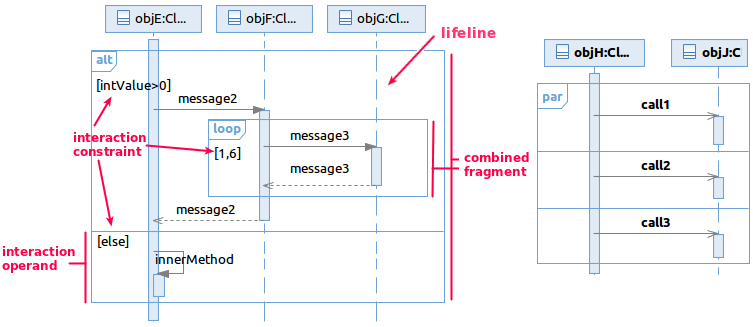
\includegraphics[width=1.0\linewidth,keepaspectratio=true]{./Figure2_merged.png}
\caption{Sequence diagrams with combined fragments}
\label{fig:SDExample}
\end{figure}

There are also two less-known combined fragments: \emph{assert} and \emph{neg}. Their use in pracice
is limited, because their semantics described in the UML 2.0 superstructure specification~\cite{UML2.4_superstructure}
is rather vague and confusing. By default, sequence diagrams without the use of these two operators 
only reflect possible behavior, while \emph{assert} and \emph{neg} alter the way 
a trace can be classified as valid or invalid. The specification characterizes
the semantics of a sequence diagram as a pair of valid and invalid traces,
where a trace is a sequence of events or messages.
The potential problems with the UML 2.0 assertion and negation are explained in~\cite{Harel07assertand}.
In summary, the specification aims to allow depicting required and forbidden behaviors.
However, as they point out, stating that ``the sequences of the operand of the assertion are the only valid continuations. All other continuations result in an invalid trace''
suggests that the invalid set of traces for an \emph{assert} fragment is its complement, i.e., the set of all other possible traces.
On the other hand, the standard declares that the
invalid set of traces are associated only with the use of
a \emph{neg} fragment, which is contradictory.
For this reason, we also believe that these two operators should rather be considered 
as modalities. We restrict their usage single events in property specifications, and assign the following semantics:
\emph{neg} is considered a set-complement operator for the event captured by the fragment, while \emph{assert}
specifies that an event must occur. In addition, we
disallow nestings between these two fragments.
We find that this does not limit the expressiveness of property specifications in practice.
% I cannot find a counter-example where it would
\section{The Approach}
\label{sec:Approach}

\subsection{The Rationale}
To describe our proposal to a correct and straightforward property elucidation,
we outline the motivations behind the choices we made, and how they differ from
existing related approaches. As already stated, to bridge the gap between everyday practical software 
requirements specification and the the property patterns classification,
several conversational tools have already been proposed. 

While we follow 
on the idea of using a guiding questionnaire to incrementally refine various aspects
of a requirement, we find the resulting artifacts from using the available ones 
not yet suitable for practical application in our context.
For one, the practitioner must manually define the events to be associated with the placeholders when 
instantiating the template. To avoid potential errors, as well as
reduce effort in specifications, we want to ideally stay in the same IDE used
for modeling the system, and select only existing events that represent
valid communication between components.  
In addition, we can already obtain~\cite{DBLP:dblp_conf/nfm/RemenskaTWHVCB13} mCRL2 models from UML designs comprising sequence diagrams.
In our experience, visual scenarios are the most suitable and commonly used  
means to specify the dynamics of a system. 
We believe that such a visual depiction of a scenario, more than finite state machines, 
improves the practitioner's understanding of the requirement as well. 
This is why we chose sequence diagrams as a property specification artifact too.

Most of the invented notations used by existing scenario approaches can fit well in UML 2.0 sequence diagrams.
Profiles are a standard way to extend UML for expressing concepts not included in the official metamodel. 
In short, UML profiles consist of stereotypes that can be applied to any UML model, like classes,
associations, or messages. We used this mechanism 
to apply the restrictions on the usage of \emph{neg} and \emph{assert},
as well as to distinguish between events presenting interval bounds and regular ones, from the patterns.
Fig.~\ref{fig:ResponsePattern} depicts the \emph{precedence chain} pattern (with
a \emph{between-Q-and-R} scope), with the stereotypes applied to messages
\emph{Q} and \emph{R}.
The pattern expresses that event \emph{P} must precede the chain of events
\emph{S, T}, always when the system execution is in the scope between events
\emph{Q} and \emph{R}.
We find this a much more intuitive scenario representation than the CHARMY/PSP
one (Fig.~\ref{fig:ResponsePatternCharmy}), for the same pattern.
Notice that we do not have to specify constraints on past unwanted events, as they are automatically
reflected in the $\mu$-calculus formula, as long as there is a distinction between interval-marking messages,
regular, mandatory, and forbidden ones. Also, their notation presents the scenario in a negative form, using ``f:'' to
explicitly mark an error message. 
\begin{figure*}[t!]
  \centering
  \subfloat[Sequence Diagram with monitor]{\label{fig:ResponsePattern}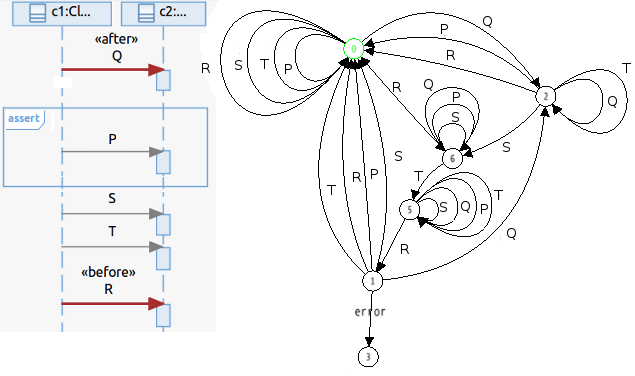
\includegraphics[width=0.62\linewidth]{./ResponseChain_withMonitor.png}}    
  \hfill
  \subfloat[PSC with Buchi automaton]{\label{fig:ResponsePatternCharmy}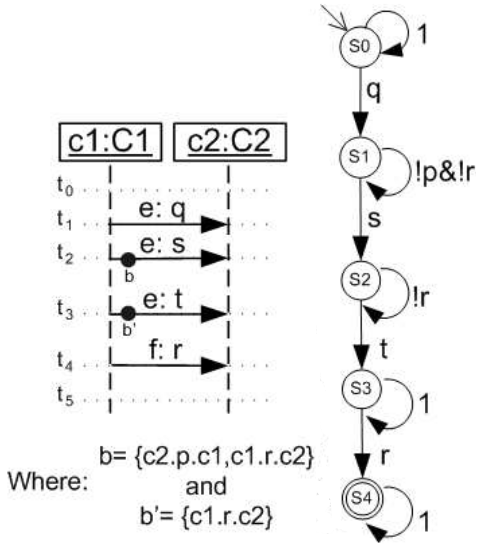
\includegraphics[width =0.38\linewidth]{./ResponseChainPSC.png}}
  \caption{Scenarios for the precedence chain pattern}
\end{figure*}
Although any mature visual UML modeling tool 
can be used, we chose IBM's RSA environment~\cite{terry2006visual}.
One of the advantages is that RSA is built on top of Eclipse, making 
it relatively easy to extend the functionality. To this end, PASS is developed as an Eclipse plugin, using the 
lightweight UML Profile, and as such is available to any Eclipse-based UML tool.

Furthermore, most visual scenario approaches cover the (state-based) LTL mappings and extensions of the pattern system. 
Event-based temporal logics have not received much attention. Even though the original pattern 
system does not cover $\mu$-calculus, such mappings~\cite{RAFMC} have been developed by the CADP team.
However, there are no pattern extensions available. These are adequate for action- or event-based systems,
making them a good match for sequence diagrams, where communication between components is depicted.
LTL logic is interpreted over Kripke structures, where the states are labeled with elementary 
propositions that hold in each state, while $\mu$-calculus is interpreted over LTS, in which the transitions
are labeled with actions that represent state changes.
Even though both are complementary representations of the more general finite state automata, 
conversions between them are not practical, as they usually lead to a significant state space increase. 
For example, the fact that a lock has
been acquired or released can be naturally expressed by actions. Since state-based
temporal logics lack this mechanism, an alternative is to introduce a variable to indicate
the status of the lock, i.e., expose the state information. With such properties, LTS
representations are more intuitive, and easier to query using event-based logics.

Given that communication among components proceeds via actions (or events) which can
represent synchronous or asynchronous communication, property specification
can be defined over sequences of actions that are data-dependent.
Fortunately, $\mu$-calculus is rich enough to express both state and action formulas,
and provides means for quantification over data, which other formalisms lack. 
%maybe this can go to the questionnaire?
For example, with our approach, a practitioner can use 
a wild-card ``*'' to express that the property should be evaluated for all values
that message parameters can carry. This allows us to use patterns which would otherwise
make sense only for state-based formalisms. For example, the \emph{universality}
pattern is used describe a portion of the system's execution which contains only states/events that have a desired property.
Checking if a certain event is executed in every step of the system execution is not useful,
so we adapted it in the context of $\mu$-calculus. 

Finally, for the purpose of on-the-fly verification, we provide an
automatically generated mCRL2 monitor which corresponds to the property formula.
We interpret a sequence diagram as an observer of
the message exchanges in the system. This helps in avoiding generation of those
parts of the state space for which it is certain that they do not compose with the
property monitor. In addition, although mcRL2 offers direct model checking
$\mu$-calculus and can provide feedback when the property fails to hold, this
feedback is not at the level of the mCRL2 process specification.
Using the monitor, the counter-example will be provided at the UML level.

\subsection{Transforming a $\mu$-calculus Formula Into a Monitor Process} 
A general model checking mechanism used with tools like SPIN 
is to construct a Buchi automaton for an LTL formula, which accepts exactly those executions
that violate the property. A product of the model state space (typically a Kripke structure) and the Buchi automaton is then composed, 
and checked for emptiness. 
Although syntactically Buchi is similar to the finite state monitor for which we aim,
the difference is in the acceptance conditions: a monitor accepts only 
finite runs of the system, while Buchi can trap infinite executions through
detection of cycles, but needs the entire state-space
generated in the process. Runtime verification
does not store the entire state space of a model, so it cannot detect such cycles. 
In addition, to expose state information, transitions in Fig.~\ref{fig:Buchi} are labeled with elementary
propositions rather than actions (notice the $\wedge$ operator). 
As such, we cannot use existing tools for constructing Buchi automata with our
approach.
\begin{figure}[!t]
\centering
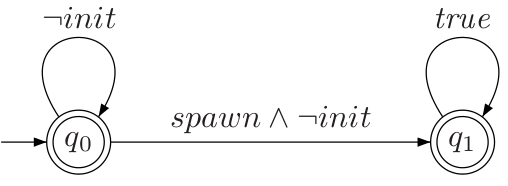
\includegraphics[width=0.4\linewidth,keepaspectratio=true]{./Buchi.png}
\caption{A Buchi automaton~\cite{Bauer:2011:RVL:2000799.2000800}}
\label{fig:Buchi}
\end{figure}

Not every property can be monitored at runtime when only a finite run has been 
observed so far. Monitorable properties are those for which a violation occurs along a finite execution.
This problem has been studied~\cite{DBLP:journals/corr/abs-1006-3638}, and it is known that the class of 
monitorable properties is strictly larger than the commonly believed class of \emph{safety} properties.
However, an exact categorization of monitorable properties is missing.
In particular, the definition of \emph{liveness} requires that any finite system
execution must be extendable to an infinite one that satisfies the property. 
On the other hand, by defining a scope of a property, we can also assert
violations to \emph{existence} patterns, which are typically in the \emph{liveness} category. 
Such runtime monitor can also assert \emph{universality} and \emph{absence} patterns 
with or without a scope combinations. We found that we are able to construct 
a monitor for about 50\% of the property patterns.

We translate a fragment of the $\mu$-calculus to mCRL2 processes which
can subsequently serve as an observer processes for monitorable properties.
We restrict to the following grammar:
\[
\begin{array}{ll}
\phi_1 & ::= b \mid \forall d:D.\phi_1 \mid [R]\phi_1 \mid \phi_1\wedge \phi_2\\
R_1,R_2 & ::= \alpha \mid nil \mid R_1\cdot R_2 \mid
              R_1+R_2 \mid
              R_1^* \mid R_1^+ \\
\alpha_1,\alpha_2 & ::= b \mid \a{a(e)} \mid \neg \alpha_1 \mid
              \alpha_1 \wedge \alpha_2 \mid
              \exists d:D.\alpha_1
\end{array}
\]
Before we present the translation, we convert the formulas in
guarded form. That is, we remove every occurrence of $R^*$ and $nil$ using
the following rules:
\[
\begin{array}{ll}
~
[nil]\phi &= \phi \\
~[R^*]\phi &= [nil]\phi \wedge [R^+]\phi
\end{array}
\]
The function $\Tr$ takes two arguments (a formula and a list of typed
variables) and produces a process. It is defined inductively as follows:
\[
\begin{array}{ll}
\Tr_l(b) &= (\neg b \to \a{error}) \\
\Tr_l(\forall d:D.\phi_1) & = \sum d:D. \Tr_{l\concat [d:D]} (\phi_1) \\
\Tr_l(\phi_1 \wedge \phi_2) & = \Tr_l(\phi_1) + \Tr_l(\phi_2) \\
\Tr_l([R]\phi_1) & = \TrR_l(R) \cdot \Tr_l(\phi) \\
\end{array}
\]
where $\TrR$ takes a regular expression (and a list of typed variables)
and produces a process or a condition:
\[
\begin{array}{ll}
\TrR_l(\alpha) &= \bigoplus\limits_{a \in Act} (\sum d_a:D_a.~ \TrA_l(a(d_a),\alpha) \to a(d_a)) \\
\TrR_l(R_1 \cdot R_2) & = \TrR_l(R_1) \cdot \TrR_l(R_2) \\
\TrR_l(R_1 + R_2) &= \TrR_l(R_1) + \TrR_l(R_2) \\
\TrR_l(R_1^+) & = X(l) \qquad \textit{where $X(l) = \TrR_l(R_1)\cdot X(l)$ is
a recursive process} 
\end{array}
\]
where $\bigoplus$ is a finite summation over all action names
$a \in Act$ and
where $\TrA$ takes an action and an action formula and produces a condition
that describes when the action is among the set of actions described by
the action formula:
\[
\begin{array}{ll}
\TrA_l(a(d_a),b) & = b \\
\TrA_l(a(d_a),a'(e)) & = \left \{ \begin{array}{ll} d_a = e & \text{if a = a'}\\
                                  \text{false} & \text{otherwise}\\
                                  \end{array} \right .\\
\TrA_l(a(d_a),\neg \alpha_1) & = \neg \TrA_l(a(d_a),\alpha_1) \\
\TrA_l(a(d_a),\alpha_1 \wedge \alpha_2) & =
\TrA_l(a(d_a),\alpha_1) \wedge \TrA_l(a(d_a),\alpha_2) \\
\TrA_l(a(d_a),\exists d:D.\alpha_1) & = \exists d:D. \TrA_l(a(d_a),\alpha_1)
\end{array}
\]
Using the above translation, Fig.~\ref{fig:ResponsePattern} shows monitor visualization next to the sequence diagram for the chain response pattern.
Such a monitor can be placed in parallel a the system model,
to perform runtime verification. Clearly, in the ``worst'' case, if the model is correct with respect to the property,
all model states will be traversed. In practice however, refutation can be found 
quickly after a limited exploration. 

\subsection{The Wizard} 
%mention free drawing and the profile application 
%mention The syntax of the µ-calculus consists of multiactions, action formulas, regular formulas and state formulas.
% this is why we CAN describe state formulas with mu-calculus!
% The last part of the property (i.e. “the withdraw request is allowed only
% after the login request and only until the logout request”) it is easily rec-
% ognized as a scope. The Scope Selection Engine proposes the different
% choices and the user is then guided to choose the “After-Until” scope
% (i.e. “After login” and “Until logout” scope) that embraces the withdraw
% request and the DB update. ← for paper!
% 
% This instantiated sentence can then be mapped to a temporal logic
% representation. The following temporal logic property, automatically generated
% by SPIDER, denotes the LTL representation of the property captured in natural
% language in Expression (6), which can be analyzed by the model checker Spin
% Fantechi et al. [9] use natural language constructs that map directly into ACTL,
% an action-based variant of CTL. User input is used to resolve ambiguities that
% might be encountered in the input phrase. 
% 
% DNL is a restricted subset of natural language that is intended to capture
% meanings unambiguously. This representation is not intended to stand by itself;
% it is meant to be used in conjunction with the FSA template representation. Like
% FSA templates, DNL templates are designed to elucidate the decisions associated
% with a property pattern. Therefore, the same options that must be decided in the
% FSA template are options in the DNL template representation. A
% fially-instantiated DNL template results in a paragraph of natural language text
% that is grammatically correct, readable, and maps to one, and only one,
% fully-instantiated FSA property. The relationship between the options in a
% pattern's DNL template and those in a pattern's FSA template is not necessarily
% one-to-one, however, since some DNL options affect the FSA templates in more
% than one location.
% 
% We illustrate how a property pattern is represented as an FSA template using the
% Response pattern. As noted above, the Response pattern is concerned with
% expressing the concept of a stimulus event that must be followed by a response
% event. An example of this property pattern as written in natural language might
% look something like this: After the elevator button is pushed, the elevator
% closes its doors. Questions arise: for example, should the doors close
% repeatedly if the button is pushed repeatedly? What, if anything, is allowed to
% occur after the button is pushed, but before the doors are closed? We find that
% these questions can be captured by using the extended FSA property notation with
% six options. These options in the Response pattern template combine to produce a
% total of sixty-four distinct variations on this property pattern. When all of
% the options have been decided, an FSA that represents only one of the sixty-four
% possible variations is created. The six Response pattern template options are as
% follows: 
% Pre-arity, which determines whether action may occur one time or many times
% before response does; Post-arity, which determines whether response may occur
% one time or many times after action does; Immediacy, which determines whether or
% not other intervening events may occur between action and response; Precedency,
% which determines whether or not response is allowed to occur before the first
% occurrence of action; Nullity, which determines whether or not action must ever
% occur; and Repeatability, which determines whether or not occurrences of action
% after an occurrence of response are required to be followed by response. Since
% we assume that the alphabet may include more events than just action and
% response, Immediacy deals with whether or not these other events may occur at
% the second state
% 
% for paper: Scopes are introduced in FVS in the same way as any
% other restriction of behavior. Thus, Global scope is implicity
% modeled by introducing no scope restrictions (all the rules
% shown up to here assumed Global scope). In what follows we
% model the rest of the scopes for the basic Response pattern2 .
% 1) Before P - After Q: The rule in figure 6-a corresponds
% to the Before P scope. The occurrence of the property must
% precede the first occurrence of P. This is, if an Action event
% occurs before the first P occurrence, then a Response event
% must also occur before P. Similarly, the scenario in figure 6-b
% shows the After Q scope. That is, if an Action event occur
% after the first Q occurrence, then a Response event must also
% occur afterwards.


\section{Case Study: DIRAC's Executor Framework revisited}
\label{sec:CaseStudy}
\section{Conclusions and future work}
\label{sec:Conclusions}

%compositional patterns
\bibliographystyle{splncs} 
\bibliography{FM2014}
\end{document}


